\section{Industry 4.0 and DT}

In most industries, the development of Digital Twins is linked
to the concept of Industry 4.0, i.e. the implementation of Digital Twin concepts
, i.e. mirroring, shadowing and threading, is linked to or integrated with Industry 4.0 concepts
such as the Internet of Things (IoT), cyber-physical systems (CPS), artificial intelligence (AI) and others.
Today, any new implementation of digital twins should include one or more Industry 4.0 concepts.\cite{pires2019digital} \\

\subsection{DT and CPS}

Cyber-physical systems integrate cyberworld and dynamic physical worlds in a multi-dimensional and complex manner. CPS provide real-time sensing, information feedback, dynamic control and other services through the integration and collaboration of computing, communication and control, known as the "3Cs".\cite{alam2017c2ps}
\\ Another concept associated with cyber-physical integration is the Digital Twin. A DT simulates real-world behaviour and provides feedback by creating high-fidelity virtual models of physical objects in virtual space.
A DT reflects a bidirectional dynamic mapping process, breaking product lifecycle boundaries and providing a complete digital footprint of products.\cite{alam2017c2ps}
This allows companies to predict physical problems earlier and with greater accuracy, to optimise the manufacturing process and to produce better products.\cite{alam2017c2ps}

\begin{figure}[h]
    \centering
    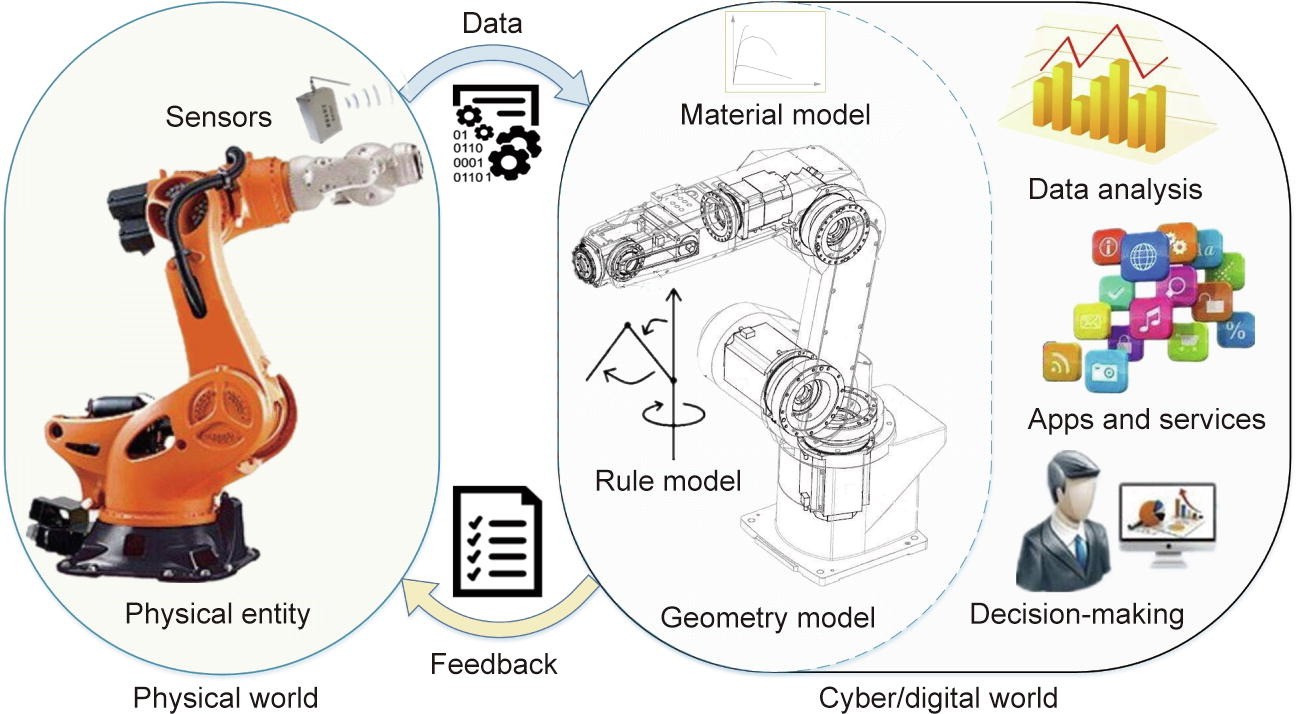
\includegraphics[width=0.6\textwidth]{CPS_DT}
    \caption{Integration of CPS and DTs}
    \label{fig:mesh2}
\end{figure}

\newpage

\subsection{DT and IoT}

Nowadays, we can connect physical objects remotely, accessing sensor data remotely, controlling the physical world remotely. The
Internet of Things (IoT) is a concept which aims to combine data collected with data obtained from
from other sources.\cite{arnarson2019digital}
\\ The Internet of Things is an essential part of Industry 4.0. It is a means of communication between people, machines and products. 
One approach to the establishment of communication is \textbf{OPC UA}.\cite{arnarson2019digital}
\\ OPCUA makes it easier to connect the digital twin to the physical twin with a third application. This could be to control and monitor the system.\cite{overn2018industry}
It also allows the system to be centralised to create a main server to which more digital twins and physical twins can be connected.\cite{overn2018industry}

\begin{figure}[h]
    \centering
    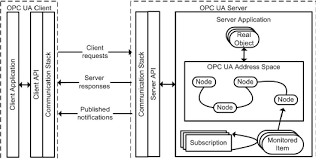
\includegraphics[width=0.9\textwidth]{opcua_server}
    \caption{OPC Unified Architecture }
    \label{fig:mesh3}
\end{figure}
